\section{Necessary Tools and Materials}

In this section we present the necessary tools and materials for the construction and assembly of the different robot hand parts. All tools and materials used, can be easily found in hardware stores around the world.

\begin{center}
\begin{tikzpicture}
\node [mybox] (box){
	\begin{tabular}{ c c }
		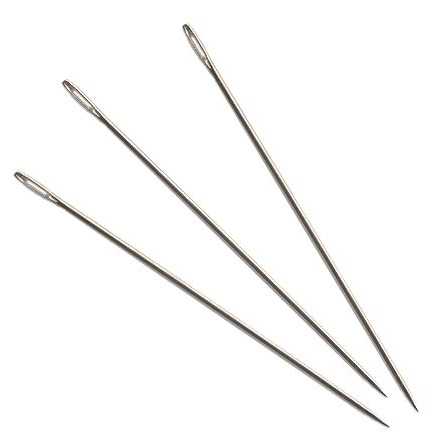
\includegraphics[width=2cm]{figures/Tools/needles.jpg} &
		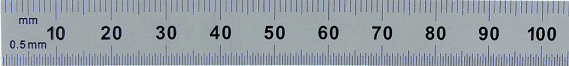
\includegraphics[width=5cm]{figures/Tools/ruler.png} 
		\\
		Long Darners [D:1mm, L:70mm] & Precision Ruler
		\\
		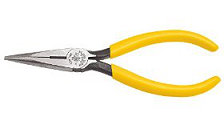
\includegraphics[width=3cm]{figures/Tools/NeedleNosePliers.png} &
		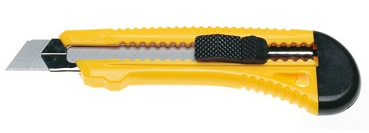
\includegraphics[width=4cm]{figures/Tools/Cutter.jpg} 
		\\
		 Long-Nose Pliers with Side-Cutting & Cutter
		\\
		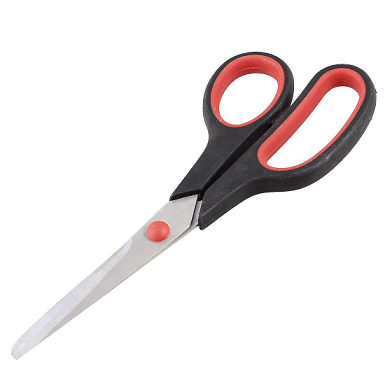
\includegraphics[width=3cm]{figures/Tools/scissors.png} &
		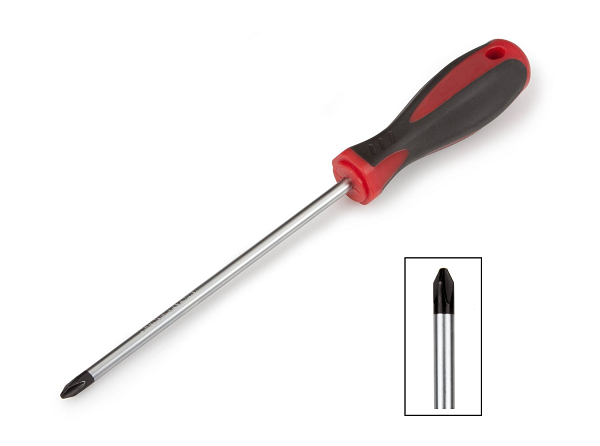
\includegraphics[width=4cm]{figures/Tools/ScrewDriver.png}
		\\
		Scissors & Phillips Screwdriver [no. 1,2]
		\\
		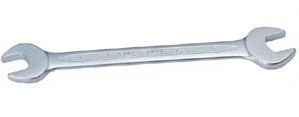
\includegraphics[width=3cm]{figures/Tools/Open-endWrench.jpg} &
		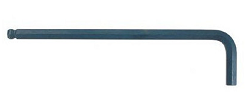
\includegraphics[width=4cm]{figures/Tools/AllenWrench.png}
		\\
		Open-End Wrench [M2, M3 Hex Nut] & Allen Wrench [2.5mm]		
		\\
    	\end{tabular}
};
\node[mytitle, right=10pt] at (box.north west) {Tools};
\end{tikzpicture}%
\end{center}

\begin{center}
\begin{tikzpicture}
\node [mybox] (box){
	\begin{tabular}{ c c c }
		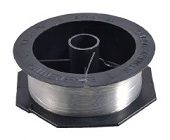
\includegraphics[width=2.0cm]{figures/Tools/FishingLine.jpg} &
                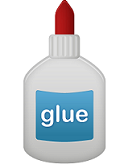
\includegraphics[width=1.5cm]{figures/Tools/Glue.jpg} &
                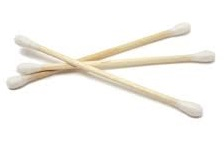
\includegraphics[width=2.5cm]{figures/Tools/Swabs.jpg}\\
		Dyneema Fishing Line [0.4mm] & Acrylic Glue \& Super Glue & Ear Cotton Swabs\\
		\& Nylon Fishing Line [0.4mm] & & \\
		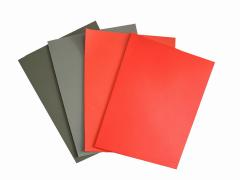
\includegraphics[width=2.5cm]{figures/Tools/Silicone.jpg} &
                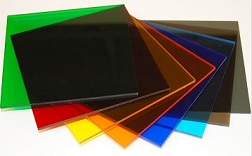
\includegraphics[width=2.5cm]{figures/Tools/Plexiglas.jpg} & 
                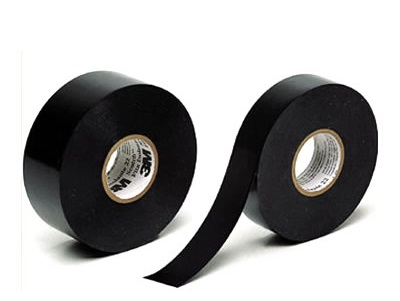
\includegraphics[width=2.5cm]{figures/Tools/Tapes.jpg}
                \\
		Silicone Sheets [3mm, 4mm] & Plexiglas Sheets [2mm, 4mm] & Sponge, Self-Adhesive \\
		& & \& Anti-Slip Tapes \\
    	\end{tabular}
};
\node[mytitle, right=10pt] at (box.north west) {Materials};
\end{tikzpicture}%
\end{center}
